\documentclass[pdflatex,sn-mathphys-num]{sn-jnl}

\usepackage{graphicx}
\usepackage{multirow}
\usepackage{amsmath,amssymb,amsfonts}
\usepackage{amsthm}
\usepackage{booktabs}
\usepackage{algorithm}
\usepackage{algorithmicx}
\usepackage{algpseudocode}
\usepackage{xcolor}

\newcommand{\rupee}{\text{Rs.}}

\graphicspath{{figures/}}

\theoremstyle{thmstyleone}
\newtheorem{theorem}{Theorem}
\newtheorem{proposition}[theorem]{Proposition}

\theoremstyle{thmstyletwo}
\newtheorem{remark}{Remark}

\raggedbottom

\begin{document}

\title[P2P Energy Trading Framework with DSM]{A Comparative Analysis Framework for Peer-to-Peer Energy Trading in Community Microgrids with Demand-Side Management: Synthetic and Real-Data Validation}

\author*[1]{\fnm{Alen} \sur{Shaju}}\email{alenshaju@nsut.ac.in}
\author[1]{\fnm{Aarav} \sur{Kumar}}
\author[1]{\fnm{Anshu} \sur{Singh}}
\author[1]{\fnm{Urishita} \sur{Gupta}}
\author[1]{\fnm{VSKV} \sur{Harish}}\email{vskvharish@ieee.org}

\affil*[1]{\orgdiv{Department of Electrical Engineering}, \orgname{Netaji Subhas University of Technology (NSUT)}, \orgaddress{\city{New Delhi}, \country{India}}}

\abstract{This paper presents a modular comparative analysis framework for evaluating peer-to-peer (P2P) energy trading mechanisms in community microgrids with integrated demand-side management (DSM). Five settlement strategies---conventional billing, Bill Sharing Mechanism (BSM), Mid-Market Ratio (MMR), static Supply-Demand Ratio (SDR), and SDR with DSM (SDR-DSM)---are benchmarked on identical community profiles using standardized metrics including cost savings and a fairness index quantifying consumer--prosumer equity. The SDR-DSM mechanism employs a distributed iterative algorithm to resolve the closed-loop price--demand feedback inherent in price-responsive load scheduling. Comprehensive parametric sweeps across community sizes ($N=7$ to $N=50$), prosumer fractions (30\%--90\%), tariff spreads (\rupee~1.0--7.5/kWh), and DSM aggressiveness parameters ($\alpha = 0.05$--$20.0$) demonstrate the framework's configurability. The methodology is validated using real Indian smart meter data from the CEEW household electricity consumption dataset (56 meters, 30 days, Bareilly and Mathura districts). Results show that SDR-DSM consistently achieves the highest community savings among all mechanisms tested, ranging from 7.3\% (narrow tariff spread) to 30.1\% (real data, 80\% prosumer composition), while MMR and static SDR systematically penalize prosumers ($\mathcal{F} \to 0$). Fairness under SDR-DSM ranges from $\mathcal{F} = 0.30$ (narrow tariff corridor limiting P2P value) to $\mathcal{F} \approx 1.0$ (balanced real-data community), with the primary synthetic case achieving $\mathcal{F} = 0.80$. Real-data validation confirms and strengthens synthetic findings, with SDR-DSM delivering 11.4\%--30.1\% savings across prosumer fractions of 20\%--80\%. Fairness is highest for compositions with 40\%--80\% prosumers ($\mathcal{F} = 0.93$--$1.00$), while the more imbalanced 20\% prosumer case yields $\mathcal{F} = 0.72$.}

\keywords{Peer-to-peer energy trading \and Community microgrid \and Supply-demand ratio pricing \and Demand-side management \and Fairness index \and Indian smart meter data}

\maketitle

%====================================================================
\section{Introduction}\label{sec:intro}

Global renewable generation capacity reached 4,448~GW in 2024, with photovoltaic (PV) installations accounting for 75\% of new additions~\cite{irena2025}. India's National Solar Mission targets 280~GW of solar capacity by 2030, with rooftop solar expected to contribute 40~GW~\cite{mnre2024}. As rooftop PV proliferates, community microgrids have emerged as a localized solution for coordinating distributed energy resources (DERs) through decentralized peer-to-peer (P2P) energy sharing and trading~\cite{sousa2019}. P2P trading establishes an internal electricity market where prosumers and consumers exchange energy at prices determined by aggregated community supply and demand, with continuous grid interconnection ensuring reliability~\cite{zhou2023}.

In the Indian context, distribution companies (DISCOMs) face significant challenges from growing rooftop solar penetration: reduced revenue from net-metered prosumers, grid stability concerns from bidirectional power flows, and cross-subsidization distortions~\cite{singh2021}. P2P trading within community microgrids offers a pathway to address these challenges by internalizing energy exchanges, reducing grid dependence, and creating value for all participants.

\subsection{Literature Review}

P2P energy trading systems can be classified along two dimensions: sharing architecture (centralized, decentralized, distributed) and market design (cost-sharing, auction-based, ratio-based deterministic pricing)~\cite{domenech2022}.

\textit{Cost-sharing mechanisms} such as the Bill Sharing Mechanism (BSM) pool community resources and redistribute costs based on allocation rules~\cite{long2017}. While simpler to implement, BSM produces temporally invariant prices that fail to incentivize real-time load adjustment and lack temporal granularity~\cite{zhang2018}. Sousa et al.~\cite{sousa2019} provide a comprehensive taxonomy showing that cost-sharing approaches dominate early implementations due to their simplicity but offer limited efficiency gains.

\textit{Auction-based mechanisms} require significant communication overhead and complexity, as peers must submit bids that determine market-clearing prices~\cite{huang2025, zhang2024}. Game-theoretic formulations~\cite{long2019, tushar2019} share similar complexity concerns for practical deployment. While theoretically optimal, the computational and communication burden makes these approaches challenging for small residential communities with limited infrastructure.

\textit{Ratio-based deterministic pricing} mechanisms, including Mid-Market Ratio (MMR) and Supply-Demand Ratio (SDR), derive internal prices directly from aggregate power quantities without strategic bidding~\cite{bogensperger2021, teotia2020}. However, these mechanisms can penalize high-yielding prosumers: Alfaverh et al.~\cite{alfaverh2023} demonstrated that conventional SDR pricing reduces prosumer revenues, and Dwivedi et al.~\cite{dwivedi2022} quantified revenue reductions of 8--15\% compared to direct grid export, discouraging sustained market participation.

\textit{Demand-side management integration} with P2P markets has been explored by Liu et al.~\cite{liu2017}, who proposed an energy-sharing model with price-based demand response for prosumer microgrids. Kanakadhurga and Padmanaban~\cite{kanakadhurga2024} combined SDR pricing with real-time pricing and double auctions in a 4-home microgrid. Jia et al.~\cite{jia2023} developed a receding-horizon approach with interval matching under uncertainty. However, these works typically address pricing, DSM, or fairness concerns in isolation rather than providing a unified framework for systematic comparison.

\textit{Real-data validation} remains a significant gap in P2P trading literature. Most studies rely exclusively on synthetic load profiles~\cite{liu2017, alfaverh2023, long2017}, which may not capture the heterogeneity and stochasticity of real household consumption patterns, particularly in developing-country contexts where load profiles differ substantially from European or North American patterns.

Table~\ref{tab:literature} summarizes significant recent works, highlighting the gap in unified comparative frameworks with real-data validation.

\begin{table*}[t]
\caption{Summary of Significant Works on P2P Energy Trading}
\label{tab:literature}
\centering
\footnotesize
\begin{tabular}{p{2.5cm}p{2.2cm}p{2.5cm}p{1.2cm}p{1.8cm}p{1.5cm}p{2.5cm}}
\toprule
\textbf{Source} & \textbf{Market Model} & \textbf{Pricing} & \textbf{DSM} & \textbf{Fairness} & \textbf{Real Data} & \textbf{Test System} \\
\midrule
Liu (2017)~\cite{liu2017} & Centralized & SDR-based & Yes & No & No & China Southern Grid \\
Long (2017)~\cite{long2017} & Community & Bill sharing & No & No & No & IEEE test feeder \\
Alfaverh (2023)~\cite{alfaverh2023} & Distributed & Dynamic SDR & Yes & Partial & No & 10-home community \\
Jia (2023)~\cite{jia2023} & Receding-horizon & Interval + CVaR & Yes & No & No & IEEE 13 \& 123 bus \\
Kanakadhurga (2024)~\cite{kanakadhurga2024} & Residential & SDR + DA & Yes & No & No & 4-home microgrid \\
Veeraswamy (2024)~\cite{veeraswamy2024} & Distributed & Mid-Market Rate & No & No & No & Residential community \\
\textbf{This work} & \textbf{Distributed} & \textbf{5 mechanisms} & \textbf{Yes} & \textbf{Yes} & \textbf{Yes} & \textbf{N=7--50, 56 real meters} \\
\bottomrule
\end{tabular}
\end{table*}

\subsection{Contributions}

The present work makes the following contributions:
\begin{enumerate}
    \item A \textit{modular comparative analysis framework} evaluating five P2P settlement mechanisms (Conventional, BSM, MMR, static SDR, SDR-DSM) on identical community profiles using standardized metrics (community cost savings and a fairness index quantifying consumer--prosumer equity).
    \item Integration of \textit{price-responsive DSM with SDR pricing} through a distributed iterative algorithm with damped updates, resolving the closed-loop price--demand feedback that static formulations cannot address, with formal convergence characterization.
    \item \textit{Comprehensive parametric analysis} across community sizes ($N=7$--$50$), prosumer fractions (30\%--90\%), tariff spreads (\rupee~1.0--7.5/kWh), and DSM aggressiveness ($\alpha = 0.05$--$20.0$), demonstrating framework configurability.
    \item \textit{Real-data validation} using Indian smart meter data from the CEEW household electricity consumption dataset (56 meters, 30 days, 15-minute resolution), confirming that synthetic findings generalize to real consumption patterns.
\end{enumerate}

%====================================================================
\section{System Model}\label{sec:system}

\subsection{Community Microgrid Architecture}

Consider a community microgrid with $N$ households comprising PV prosumers $\mathcal{P}$ and pure consumers $\mathcal{C}$, where $\mathcal{N} = \mathcal{P} \cup \mathcal{C}$. An Energy Service Provider (ESP) acts as the central coordinator for market clearing and settlement, maintaining communication links with all participants and the utility grid interconnection point. The community operates grid-connected, ensuring reliability through continuous utility backup.

The simulation horizon spans $H$ discrete time slots of duration $\Delta t$ hours. For household $n \in \mathcal{N}$ at time slot $t$, the net power is:
\begin{equation}
    P_{n,t}^{\text{net}} = D_{n,t} - G_{n,t}
    \label{eq:net_power}
\end{equation}
where $D_{n,t}$ is the electricity demand and $G_{n,t}$ is PV generation (with $G_{n,t} \equiv 0$ for consumers $n \in \mathcal{C}$). Self-consumption, import, and export powers are:
\begin{equation}
    P_{n,t}^{\text{self}} = \min(D_{n,t},\; G_{n,t})
    \label{eq:self_consumption}
\end{equation}
\begin{equation}
    P_{n,t}^{\text{im}} = \max(P_{n,t}^{\text{net}},\; 0), \quad P_{n,t}^{\text{ex}} = \max(-P_{n,t}^{\text{net}},\; 0)
    \label{eq:import_export}
\end{equation}

Community aggregate import and export at time $t$ are:
\begin{equation}
    P_t^{\text{buy}} = \sum_{n \in \mathcal{N}} P_{n,t}^{\text{im}}, \quad P_t^{\text{sell}} = \sum_{n \in \mathcal{N}} P_{n,t}^{\text{ex}}
    \label{eq:community_aggregate}
\end{equation}

\subsection{Grid Tariff Structure}

The grid buying tariff $\pi^{\text{buy}}$ and selling tariff $\pi^{\text{sell}}$ define the upper and lower bounds for internal P2P prices. In the Indian context, $\pi^{\text{buy}}$ corresponds to the DISCOM retail supply rate and $\pi^{\text{sell}}$ to the feed-in tariff for rooftop solar. Community-level reference tariffs are:
\begin{equation}
    \bar{\pi}^{\text{buy}} = \frac{1}{N}\sum_{n=1}^{N}\pi_n^{\text{buy}}, \quad \bar{\pi}^{\text{sell}} = \frac{1}{|\mathcal{P}|}\sum_{n \in \mathcal{P}}\pi_n^{\text{sell}}
    \label{eq:ref_tariffs}
\end{equation}

The ESP derives revenue from a service fee proportional to locally traded energy:
\begin{equation}
    S^{\text{ESP}} = \beta \sum_{t=1}^{H} \min(P_t^{\text{sell}},\; P_t^{\text{buy}}) \cdot \Delta t
    \label{eq:esp_revenue}
\end{equation}
where $\beta$ covers metering, communication, settlement, and distribution losses.

\subsection{Performance Metrics}

Community savings relative to conventional billing:
\begin{equation}
    \text{CS} = \frac{B^{\text{conv}} - B^{\text{P2P}}}{|B^{\text{conv}}|} \times 100\%
    \label{eq:community_savings}
\end{equation}

Group-level cost deltas for consumers and prosumers:
\begin{equation}
    \Delta_{\mathcal{C}} = \frac{B_{\mathcal{C}}^{\text{conv}} - B_{\mathcal{C}}^{\text{P2P}}}{|B_{\mathcal{C}}^{\text{conv}}|} \times 100\%, \quad \Delta_{\mathcal{P}} = \frac{B_{\mathcal{P}}^{\text{conv}} - B_{\mathcal{P}}^{\text{P2P}}}{|B_{\mathcal{P}}^{\text{conv}}|} \times 100\%
    \label{eq:group_deltas}
\end{equation}

The fairness index quantifies equity between participant groups:
\begin{equation}
    \mathcal{F} = 1 - \frac{|\Delta_{\mathcal{C}} - \Delta_{\mathcal{P}}|}{|\Delta_{\mathcal{C}}| + |\Delta_{\mathcal{P}}| + \varepsilon}
    \label{eq:fairness}
\end{equation}
where $\varepsilon$ is a small constant for numerical stability. $\mathcal{F} = 1$ when both groups benefit equally; $\mathcal{F} \to 0$ when one group's gain comes entirely at the other's expense.

%====================================================================
\section{P2P Pricing Mechanisms}\label{sec:mechanisms}

\subsection{Bill Sharing Mechanism (BSM)}

The BSM pools community resources over the billing period and computes constant ex-post prices. Total community import and export energies are:
\begin{equation}
    E^{\text{buy}} = \sum_{t=1}^{H} P_t^{\text{buy}} \cdot \Delta t, \quad E^{\text{sell}} = \sum_{t=1}^{H} P_t^{\text{sell}} \cdot \Delta t
    \label{eq:bsm_energy}
\end{equation}

The community's net grid interaction determines internal prices:
\begin{equation}
    \pi^{\text{int,buy}} = \frac{\bar{\pi}^{\text{buy}} \cdot E_{\text{grid}}^{\text{im}}}{E^{\text{buy}}}, \quad \pi^{\text{int,sell}} = \frac{\bar{\pi}^{\text{sell}} \cdot E_{\text{grid}}^{\text{ex}}}{E^{\text{sell}}}
    \label{eq:bsm_prices}
\end{equation}
where $E_{\text{grid}}^{\text{im}}$ and $E_{\text{grid}}^{\text{ex}}$ are the net community-level grid import and export energies. BSM produces temporally invariant prices, which while ensuring simplicity, provides no incentive for real-time load adjustment. Note that when the community is a net importer (i.e., $E_{\text{grid}}^{\text{ex}} \ll E^{\text{sell}}$), the internal selling price $\pi^{\text{int,sell}} \to 0$, meaning prosumers receive diminishing compensation for locally consumed exports. This degenerate case partially explains BSM's moderate prosumer performance in communities with high aggregate demand relative to PV generation.

\subsection{Mid-Market Ratio (MMR) Pricing}

The MMR establishes a time-varying midpoint price anchored between grid tariffs:
\begin{equation}
    \pi^{\text{mid}} = \frac{\bar{\pi}^{\text{buy}} + \bar{\pi}^{\text{sell}}}{2}
    \label{eq:mmr_mid}
\end{equation}

At each time slot, the community net balance index is:
\begin{equation}
    \eta_t = \frac{P_t^{\text{buy}} - P_t^{\text{sell}}}{P_t^{\text{buy}} + P_t^{\text{sell}}}
    \label{eq:mmr_balance}
\end{equation}

The P2P clearing price adjusts dynamically:
\begin{equation}
    \pi_t^{\text{p2p}} = \pi^{\text{mid}} + \frac{\bar{\pi}^{\text{buy}} - \bar{\pi}^{\text{sell}}}{2} \cdot \eta_t
    \label{eq:mmr_price}
\end{equation}

When community supply exceeds demand ($\eta_t < 0$), the price drops toward $\bar{\pi}^{\text{sell}}$, depressing prosumer revenues. During deficit periods ($\eta_t > 0$), the price rises toward $\bar{\pi}^{\text{buy}}$. While MMR introduces temporal variation, surplus periods can significantly depress prosumer revenues.

\subsection{Supply-Demand Ratio (SDR) Based Pricing}

The Supply-Demand Ratio captures the instantaneous balance between community supply and demand:
\begin{equation}
    \text{SDR}_t = \frac{P_t^{\text{sell}}}{P_t^{\text{buy}} + \varepsilon}
    \label{eq:sdr}
\end{equation}
where $\varepsilon$ is a small constant for numerical stability. The SDR directly indicates market conditions: $\text{SDR}_t < 1$ indicates energy shortage, $\text{SDR}_t = 1$ represents balance, and $\text{SDR}_t > 1$ signals surplus.

The internal prices are defined piecewise based on market regime. When $\text{SDR}_t < 1$ (deficit regime):
\begin{equation}
    \pi_t^{\text{int,sell}} = \frac{\bar{\pi}^{\text{buy}} \cdot \bar{\pi}^{\text{sell}}}{(\bar{\pi}^{\text{buy}} - \bar{\pi}^{\text{sell}}) \cdot \text{SDR}_t + \bar{\pi}^{\text{sell}}}
    \label{eq:sdr_sell}
\end{equation}
\begin{equation}
    \pi_t^{\text{int,buy}} = \pi_t^{\text{int,sell}} \cdot \text{SDR}_t + \bar{\pi}^{\text{buy}} \cdot (1 - \text{SDR}_t)
    \label{eq:sdr_buy}
\end{equation}

When $\text{SDR}_t \geq 1$ (surplus regime), supply exceeds demand and all excess must be exported to the grid. Both prices are clamped to the floor:
\begin{equation}
    \pi_t^{\text{int,buy}} = \pi_t^{\text{int,sell}} = \bar{\pi}^{\text{sell}}, \quad \text{if } \text{SDR}_t \geq 1
    \label{eq:sdr_clamp}
\end{equation}

This piecewise formulation ensures: (i)~price monotonicity with respect to SDR in the deficit regime, (ii)~prices strictly bounded within $[\bar{\pi}^{\text{sell}},\; \bar{\pi}^{\text{buy}}]$ across all market conditions, and (iii)~zero-arbitrage conditions. The clamping at $\text{SDR}_t \geq 1$ reflects that during surplus periods, additional local supply has no marginal value above the grid export tariff.

Energy allocation follows a priority rule: P2P energy is $E_t^{\text{P2P}} = \min(P_t^{\text{buy}}, P_t^{\text{sell}}) \cdot \Delta t$. Importing participants purchase P2P energy at $\pi_t^{\text{int,buy}}$ and any residual from the grid at $\bar{\pi}^{\text{buy}}$. Exporting participants sell P2P energy at $\pi_t^{\text{int,sell}}$ and any surplus to the grid at $\bar{\pi}^{\text{sell}}$.

\subsection{SDR with Demand-Side Management (SDR-DSM)}

Participants can adjust consumption $x_{n,t}$ in response to price signals, transforming the net power to:
\begin{equation}
    P_{n,t}^{\text{net}} = x_{n,t} - G_{n,t}
    \label{eq:dsm_net}
\end{equation}

The inconvenience of load shifting is modeled using a quadratic penalty~\cite{alfaverh2023, liu2017}:
\begin{equation}
    C_{n}^{\text{inc}} = \alpha_n \sum_{t=1}^{H} (x_{n,t} - D_{n,t}^{\text{ref}})^2 \cdot \Delta t
    \label{eq:inconvenience}
\end{equation}
where $D_{n,t}^{\text{ref}}$ is the reference (unshifted) load profile and $\alpha_n$ is the sensitivity coefficient representing tolerance to load shifting. The quadratic form penalizes large deviations disproportionately, reflecting practical reality where minor adjustments (e.g., pre-cooling) are tolerable but major shifts (e.g., deferring cooking) are increasingly inconvenient.

Each participant independently minimizes:
\begin{equation}
    \min_{x_{n,t}} \sum_{t=1}^{H} \left[ \pi_{n,t} \cdot P_{n,t}^{\text{net}} \cdot \Delta t + \alpha_n (x_{n,t} - D_{n,t}^{\text{ref}})^2 \cdot \Delta t \right]
    \label{eq:objective}
\end{equation}
subject to:
\begin{equation}
    \sum_{t=1}^{H} x_{n,t} \cdot \Delta t = \sum_{t=1}^{H} D_{n,t}^{\text{ref}} \cdot \Delta t \quad \text{(energy conservation)}
    \label{eq:energy_conservation}
\end{equation}
\begin{equation}
    0.5 \cdot D_{n,t}^{\text{ref}} \leq x_{n,t} \leq 1.5 \cdot D_{n,t}^{\text{ref}}, \quad \forall t \quad \text{(load bounds)}
    \label{eq:load_bounds}
\end{equation}

Constraint~\eqref{eq:energy_conservation} ensures only load shifting occurs (no curtailment). Constraint~\eqref{eq:load_bounds} imposes physical bounds reflecting the practical range of deferrable loads ($\pm$50\% of reference). The energy conservation is enforced on a per-day basis to prevent unrealistic inter-day energy transfers.

\subsubsection{Role of the $\alpha$ Parameter}

The discomfort coefficient $\alpha$ controls the trade-off between economic savings and user inconvenience. For given prices $\pi_{n,t}$, the unconstrained optimal adjustment scales as:
\begin{equation}
    x_{n,t}^* - D_{n,t}^{\text{ref}} \propto -\frac{\pi_{n,t}}{2\alpha_n}
    \label{eq:alpha_scaling}
\end{equation}

Small $\alpha$ produces aggressive load shifting (limited by the $\pm$50\% bounds), while large $\alpha$ produces negligible response. This parameter can represent heterogeneous household flexibility: a household with automated appliance scheduling might have $\alpha = 0.05$, while one with primarily non-deferrable loads might have $\alpha = 5.0$.

%====================================================================
\section{Distributed Settlement Algorithm}\label{sec:algorithm}

The SDR-DSM mechanism creates a feedback loop: prices depend on SDR, SDR depends on aggregate demand, and demand depends on prices. This is resolved through a distributed iterative algorithm coordinated by the ESP.

\begin{algorithm}[t]
\caption{Distributed SDR-DSM Settlement}
\label{alg:sdr_dsm}
\begin{algorithmic}[1]
\Require $D_{n,t}^{\text{ref}}$, $G_{n,t}$, $\bar{\pi}^{\text{buy}}$, $\bar{\pi}^{\text{sell}}$, $\alpha_n$, $\epsilon_{\text{conv}}$, $\gamma$
\Ensure $x_{n,t}^{*}$, $\pi_t^{\text{int,buy}}$, $\pi_t^{\text{int,sell}}$
\State Initialize $x_{n,t}^{(0)} \leftarrow D_{n,t}^{\text{ref}}$ for all $n, t$; set $k \leftarrow 0$
\Repeat
    \State ESP aggregates $P_t^{\text{sell},(k)}$, $P_t^{\text{buy},(k)}$ from $\{x_{n,t}^{(k)}\}$
    \State Compute $\text{SDR}_t^{(k)}$ via \eqref{eq:sdr}
    \State Update prices $\pi_t^{(k)}$ via \eqref{eq:sdr_sell}--\eqref{eq:sdr_buy}
    \For{each participant $n \in \mathcal{N}$}
        \State Solve \eqref{eq:objective} s.t. \eqref{eq:energy_conservation}--\eqref{eq:load_bounds} $\to \tilde{x}_{n,t}^{(k+1)}$
        \State $x_{n,t}^{(k+1)} \leftarrow (1-\gamma) x_{n,t}^{(k)} + \gamma \tilde{x}_{n,t}^{(k+1)}$ \Comment{Damped update}
    \EndFor
    \State $k \leftarrow k + 1$
\Until{$\max_n \|x_n^{(k)} - x_n^{(k-1)}\|_\infty < \epsilon_{\text{conv}}$ \textbf{or} $k = k_{\max}$}
\end{algorithmic}
\end{algorithm}

Algorithm~\ref{alg:sdr_dsm} details the procedure. The damping factor $\gamma = 0.3$ blends new solutions with previous iterates, preventing oscillatory behavior in the price--demand feedback loop. Each participant's subproblem is a convex quadratic program with a unique minimizer for given prices, ensuring well-defined updates.

\subsection{Convergence Analysis}

The iterative algorithm defines a composite mapping whose convergence properties we now establish, following the framework of Liu et al.~\cite{liu2017}.

\subsubsection{Existence of a Fixed Point}

The iterative process in Algorithm~\ref{alg:sdr_dsm} can be decomposed into two mappings:
\begin{itemize}
    \item \textit{Schedule mapping} $Y$: Given internal prices $\mathbf{Pr} = \{\pi_{n,t}\}$, each participant solves \eqref{eq:objective}--\eqref{eq:load_bounds} to obtain optimal schedules $\mathbf{x}^* = Y(\mathbf{Pr})$.
    \item \textit{Price mapping} $H$: Given schedules $\mathbf{x}$, the ESP computes aggregate quantities, SDR via \eqref{eq:sdr}, and internal prices via \eqref{eq:sdr_sell}--\eqref{eq:sdr_buy}, yielding $\mathbf{Pr} = H(\mathbf{x})$.
\end{itemize}

The composite mapping is:
\begin{equation}
    V(\mathbf{Pr}) = H(Y(\mathbf{Pr}))
    \label{eq:fixed_point}
\end{equation}

A settlement equilibrium corresponds to a fixed point $\mathbf{Pr}^* = V(\mathbf{Pr}^*)$.

\begin{proposition}\label{prop:convex}
The cost function $C_i(x_{i,t})$ in \eqref{eq:objective} is strictly convex in $x_{i,t}$ for each participant $i$ and time slot $t$, given fixed prices.
\end{proposition}

\textit{Proof.} The cost at time $t$ for participant $i$ is $C_i^t = \pi_{i,t} \cdot (x_{i,t} - G_{i,t}) \cdot \Delta t + \alpha_i(x_{i,t} - D_{i,t}^{\text{ref}})^2 \cdot \Delta t$. The first term is linear in $x_{i,t}$ (since $\pi_{i,t}$ is treated as fixed within each iteration). The second term is strictly convex with $\alpha_i > 0$. Their sum is strictly convex, and since the constraint set \eqref{eq:energy_conservation}--\eqref{eq:load_bounds} is a bounded polyhedron (hence convex and compact), the optimization has a unique minimizer. \hfill$\square$

This guarantees $Y$ is a well-defined (single-valued) function from prices to schedules. Moreover, $Y$ is continuous by the maximum theorem~\cite{berge1963}, since the objective is continuous in both $\mathbf{x}$ and $\mathbf{Pr}$ and the constraint set is constant.

\begin{proposition}\label{prop:fixed_point}
The composite mapping $V: \mathcal{D} \to \mathcal{D}$ has at least one fixed point, where $\mathcal{D} = [\bar{\pi}^{\text{sell}}, \bar{\pi}^{\text{buy}}]^H$ is the price domain.
\end{proposition}

\textit{Proof.} The domain $\mathcal{D}$ is a bounded, closed, convex subset of $\mathbb{R}^H$. The price mapping $H$ produces prices bounded in $[\bar{\pi}^{\text{sell}}, \bar{\pi}^{\text{buy}}]$ by construction of \eqref{eq:sdr_sell}--\eqref{eq:sdr_buy}, so $V: \mathcal{D} \to \mathcal{D}$. Both $Y$ (by the maximum theorem) and $H$ (by continuity of the SDR pricing formulas) are continuous, hence $V$ is continuous. By the Brouwer Fixed Point Theorem, $V$ has at least one fixed point. \hfill$\square$

\subsubsection{Practical Convergence}

\begin{remark}
Propositions~\ref{prop:convex}--\ref{prop:fixed_point} guarantee that an equilibrium exists within the bounded price domain. Algorithm~\ref{alg:sdr_dsm} converges to this equilibrium across all parameter configurations tested in this study, consistent with the findings of Liu et al.~\cite{liu2017} who observed convergence for $\alpha \geq 0.009$ in a comparable system. The combination of guaranteed equilibrium existence with empirical convergence across a broad parameter space provides a practical convergence assurance for the operating regime of interest ($\alpha \geq 0.05$, $\gamma = 0.3$).
\end{remark}

The key factor controlling convergence is the sensitivity coefficient $\alpha$: from \eqref{eq:alpha_scaling}, the optimal load adjustment to a price perturbation $\delta\pi$ scales as $\mathcal{O}(\delta\pi / (2\alpha))$. Smaller $\alpha$ produces larger demand response per price change, amplifying the feedback loop and potentially causing oscillation or divergence. Liu et al.~\cite{liu2017} demonstrated empirically that without damping, their comparable SDR-based system diverges for $\alpha < 0.009$.

The damping factor $\gamma = 0.3$ in Algorithm~\ref{alg:sdr_dsm} reduces the effective gain by blending new solutions with previous iterates, improving stability at the cost of slower convergence. Our choice of $\alpha = 0.12$ with $\gamma = 0.3$ provides a conservative stability margin.

Fig.~\ref{fig:convergence} shows the convergence trajectory for the $N=20$ primary case. Community savings increase from 6.3\% (iteration~1) to 13.5\% (iteration~8), while fairness rises from 0.0 to 0.80. The maximum inter-iteration load change stabilizes below 0.25~kW. Convergence was observed across all parameter combinations tested in this study ($N = 7$--$50$, $\alpha = 0.05$--$20.0$, spreads \rupee~1.0--7.5), with 8 iterations consistently sufficient for practical settlement.

\begin{figure}[t]
    \centering
    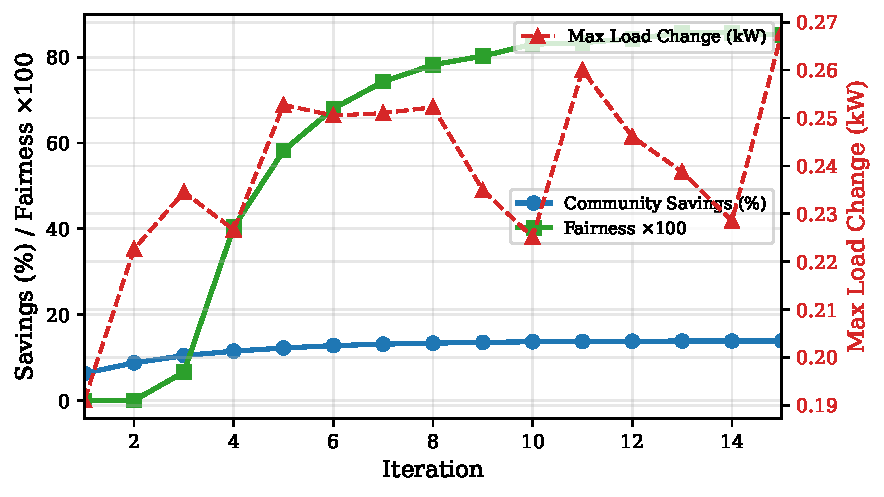
\includegraphics[width=\columnwidth]{fig_convergence.pdf}
    \caption{Convergence of the distributed SDR-DSM algorithm ($N=20$, $\alpha=0.12$, $\gamma=0.3$): maximum inter-iteration load change and community savings vs. iteration number.}
    \label{fig:convergence}
\end{figure}

%====================================================================
\section{Simulation Setup}\label{sec:setup}

\subsection{Synthetic Data Configuration}

The primary test case consists of $N=20$ households with 8 pure consumers and 12 PV prosumers (categorized as small, medium, and large PV systems). The simulation spans 30 days at 15-minute resolution ($\Delta t = 0.25$~h), yielding 96 time slots per day and 2,880 total time steps. Table~\ref{tab:params} summarizes key parameters.

\begin{table}[t]
\caption{Simulation Parameters}
\label{tab:params}
\centering
\begin{tabular}{lll}
\toprule
\textbf{Parameter} & \textbf{Value} & \textbf{Unit} \\
\midrule
Simulation duration & 30 & days \\
Time resolution ($\Delta t$) & 15 & min \\
Primary community ($N$) & 20 & -- \\
\quad Consumers & 8 & -- \\
\quad Prosumers (S/M/L) & 5/4/3 & -- \\
Consumer daily load & 4--7 & kWh/day \\
Prosumer daily load & 5--9 & kWh/day \\
PV yield & 4.5--5.5 & kWh/kWp/day \\
Grid buy tariff ($\bar{\pi}^{\text{buy}}$) & 5.8752 & \rupee/kWh \\
Grid sell tariff ($\bar{\pi}^{\text{sell}}$) & 3.2462 & \rupee/kWh \\
DSM coefficient ($\alpha$) & 0.12 & \rupee/kW$^2$ \\
Damping factor ($\gamma$) & 0.3 & -- \\
Max iterations ($k_{\max}$) & 8 & -- \\
ESP service fee ($\beta$) & 2 & \% \\
Load bounds & $\pm$50\% & of $D_{n,t}^{\text{ref}}$ \\
\bottomrule
\end{tabular}
\end{table}

Demand profiles follow a composite Gaussian shape with morning (08:00) and evening (20:00) peaks, $\pm$5\% daily variation, and per-slot noise. PV generation follows a clear-sky sinusoidal curve (06:00--18:00) with $\pm$15\% variability representing cloud cover. Prosumer PV sizing is categorized: small (40--60\% of daily load), medium (80--110\%), and large (130--180\%).

\subsection{Real Smart Meter Data}

The framework is validated using real household electricity consumption data from the CEEW (Council on Energy, Environment and Water) smart meter dataset~\cite{ceew2021} (doi:10.7910/DVN/GOCHJH), collected from residential households in Bareilly and Mathura districts of Uttar Pradesh, India during 2019--2020 at 3-minute resolution.

\subsubsection{Data Preprocessing}

The raw 3-minute data is aggregated to 15-minute intervals to match the simulation resolution. A quality filtering pipeline ensures data integrity:
\begin{enumerate}
    \item \textbf{Window selection}: The best 30-day contiguous window (2020-02-05 to 2020-03-06) is selected based on data completeness across all meters.
    \item \textbf{Coverage filtering}: Meters with $<$90\% temporal coverage within the selected window are excluded, yielding 56 usable meters from an initial pool of 83.
    \item \textbf{Gap filling}: Missing values are filled using the median profile for each meter's corresponding time-of-day slot.
    \item \textbf{Outlier capping}: Consumption values exceeding 5$\times$ the meter's median are capped to prevent unrealistic spikes from measurement artifacts.
\end{enumerate}

\subsubsection{Role Assignment and PV Generation}

Since the CEEW dataset contains only consumption data, PV systems are synthetically assigned to designated prosumers. PV capacity for each prosumer is sized proportionally to their mean daily consumption (capacity factor $= 0.8 \times$ mean daily load), generating realistic PV-to-load ratios. The PV generation profile uses the same clear-sky sinusoidal model as synthetic data, representing typical North Indian insolation patterns.

\subsection{Contingency Modeling}

Two contingency types are modeled: (i)~full-day PV outages due to inverter failure (2 events/month), and (ii)~P2P trading disruptions during communication failures (3 events of 2~hours each per month). During contingencies, affected peers settle directly with the grid at standard tariffs.

%====================================================================
\section{Results and Discussion}\label{sec:results}

\subsection{Community Aggregate Power Profiles}

Fig.~\ref{fig:aggregate} shows the community aggregate power profiles for the $N=20$ primary case. The reference load exhibits a characteristic twin-peak pattern (morning and evening), while the DSM-adjusted load shows pronounced midday advancement, aligning demand with peak PV generation. The shaded surplus region (PV exceeding adjusted demand) during 09:00--15:00 represents energy available for P2P trading and grid export. The DSM-adjusted load reduces the evening peak by approximately 15\% while increasing midday consumption by 25--30\%, demonstrating effective temporal load shifting without energy curtailment.

\begin{figure}[t]
    \centering
    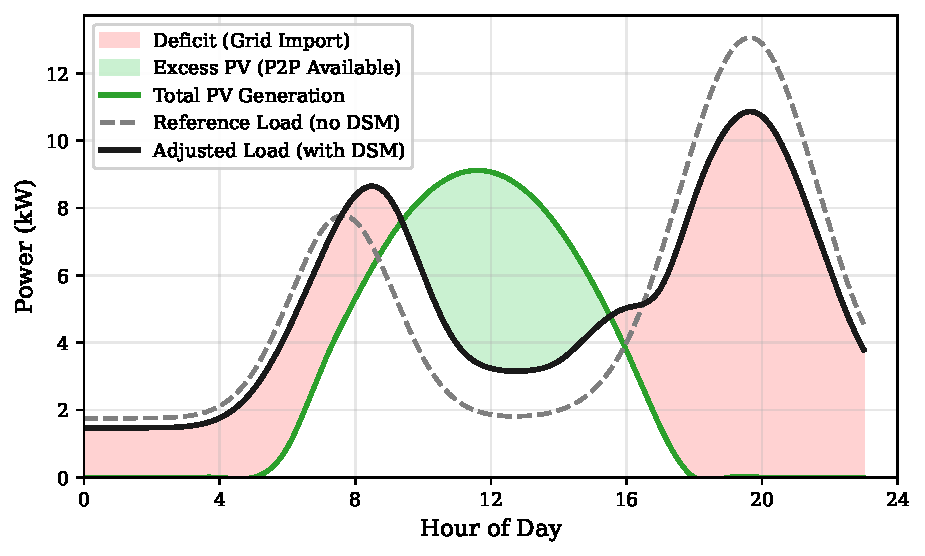
\includegraphics[width=\columnwidth]{fig_aggregate_profiles.pdf}
    \caption{Community aggregate power profiles ($N=20$): reference load, DSM-adjusted load, and PV generation with surplus/deficit shading.}
    \label{fig:aggregate}
\end{figure}

\subsection{Individual Load Reshaping}

Fig.~\ref{fig:reshaping} presents load profiles for representative participants under SDR-DSM pricing. Prosumers with large PV systems aggressively shift demand toward midday (hours 9--15) where high surplus produces low clearing prices, while reducing evening consumption. Consumers, despite lacking PV, also benefit from shifted community prices---they increase midday purchases when P2P prices are lowest. The shaded regions quantify the magnitude of DSM-induced load shifting relative to each participant's reference profile.

\begin{figure}[t]
    \centering
    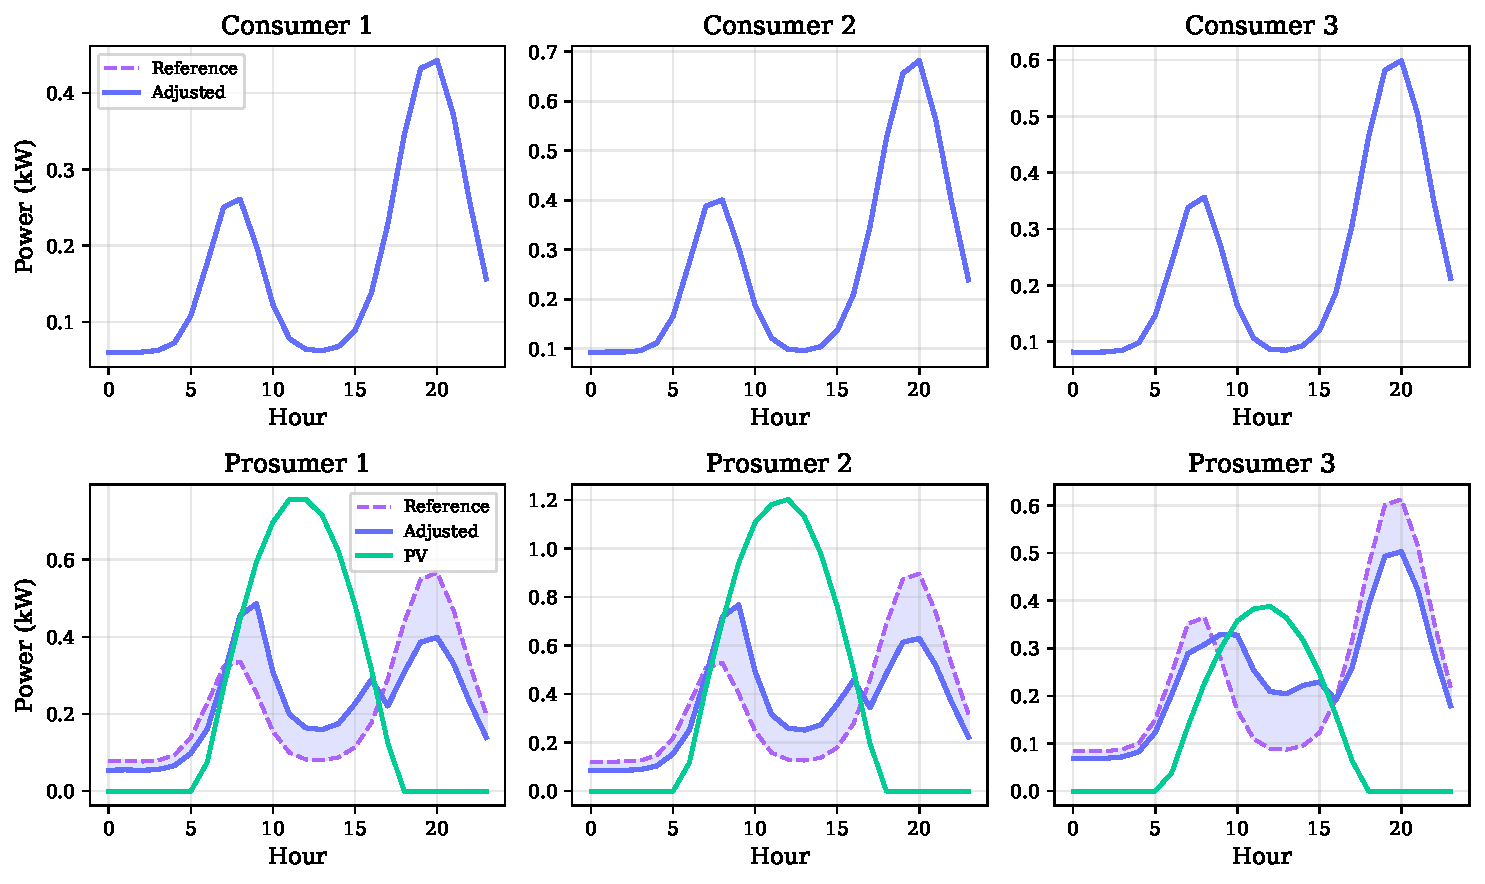
\includegraphics[width=\columnwidth]{fig_individual_reshaping.pdf}
    \caption{Individual load reshaping under SDR-DSM: reference vs. adjusted load profiles for representative prosumers and consumers with PV generation overlay.}
    \label{fig:reshaping}
\end{figure}

\subsection{SDR Dynamics and Price Formation}

The SDR variation (Fig.~\ref{fig:sdr}) divides the operational day into three distinct regimes: morning deficit ($\text{SDR}_t \ll 1$, 06:00--09:00), midday surplus ($\text{SDR}_t > 1$, peaking at approximately 16 during 10:00--14:00), and evening deficit as PV generation ceases. Under DSM, the midday SDR peak is reduced compared to the static case because increased midday demand absorbs more surplus locally.

\begin{figure}[t]
    \centering
    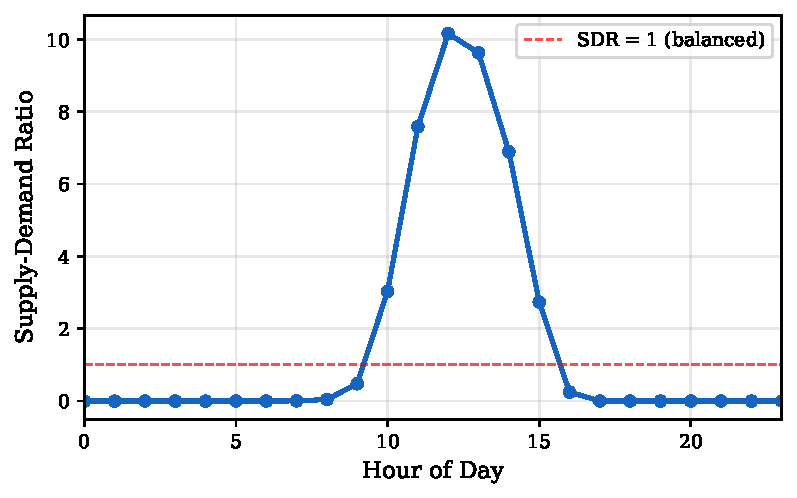
\includegraphics[width=\columnwidth]{fig_sdr_hourly.pdf}
    \caption{Hourly Supply-Demand Ratio variation showing market regime transitions: deficit (SDR$<$1), balance (SDR$=$1), and surplus (SDR$>$1).}
    \label{fig:sdr}
\end{figure}

Fig.~\ref{fig:prices_sdr} shows the corresponding P2P clearing prices under SDR-DSM. During peak PV periods, internal prices collapse from \rupee~5.88/kWh toward the export floor of \rupee~3.25/kWh, serving as the natural DSM trigger. Prices remain strictly bounded between utility tariff limits, ensuring no arbitrage opportunities.

\begin{figure}[t]
    \centering
    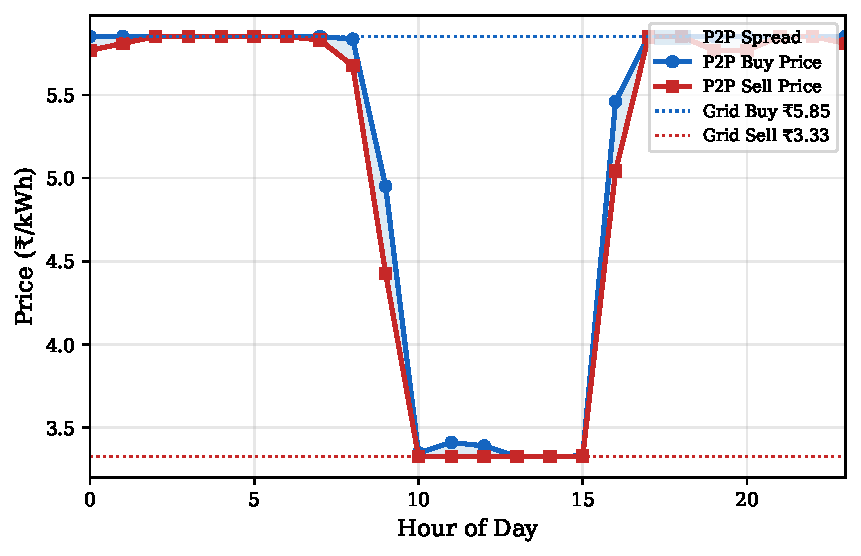
\includegraphics[width=\columnwidth]{fig_prices_sdr_dsm.pdf}
    \caption{SDR-DSM P2P clearing prices compared with grid tariff bounds, showing price collapse during surplus periods.}
    \label{fig:prices_sdr}
\end{figure}

\subsection{Comparative Price Analysis}

Fig.~\ref{fig:prices_all} compares all four P2P pricing mechanisms. BSM produces flat prices (no temporal signal). MMR generates moderate variation anchored around the midpoint (\rupee~4.56/kWh). Static SDR shows strong temporal variation but without demand feedback. SDR-DSM exhibits the most pronounced price dynamics due to the demand-response feedback loop: midday prices drop further as demand shifts absorb surplus, while deficit-period prices rise less due to reduced peak demand.

\begin{figure}[t]
    \centering
    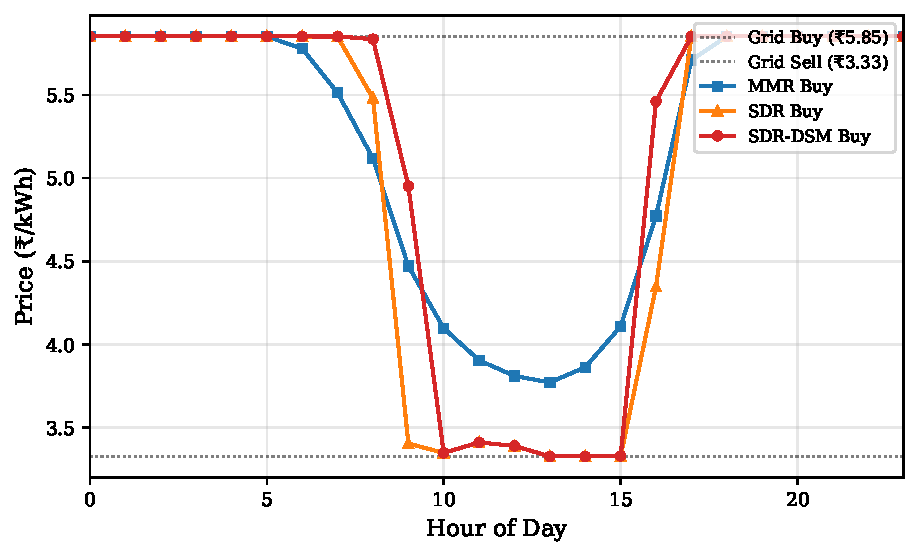
\includegraphics[width=\columnwidth]{fig_prices_comparison.pdf}
    \caption{Comparative price profiles across all four P2P mechanisms over a representative day.}
    \label{fig:prices_all}
\end{figure}

\subsection{Economic Evaluation}

Table~\ref{tab:economics} presents the 30-day economic performance for the $N=20$ primary case (8C+12P, seed=42). Under conventional billing, consumers account for 64\% of the total community cost (8 consumers purchasing all demand from the grid) while prosumers account for 36\% (12 prosumers self-consuming the majority of their PV generation, paying only for net imports). MMR achieves high consumer savings (16.41\%) but reduces prosumer revenues ($\Delta_\mathcal{P} = -5.57$\%), yielding $\mathcal{F} \approx 0$. Static SDR similarly penalizes prosumers ($\Delta_\mathcal{P} = -13.42$\%). BSM achieves moderate and relatively equitable savings ($\mathcal{F} = 0.84$). The SDR-DSM framework achieves the highest community savings (13.52\%) with $\mathcal{F} = 0.80$, benefiting both groups simultaneously: consumers save 15.33\% and prosumers gain 10.28\%.

\begin{table}[t]
\caption{30-Day Economic Performance Comparison ($N=20$, 8C+12P, seed=42)}
\label{tab:economics}
\centering
\footnotesize
\begin{tabular}{lcccc}
\toprule
\textbf{Metric} & \textbf{BSM} & \textbf{MMR} & \textbf{SDR} & \textbf{SDR-DSM} \\
\midrule
Community savings (\%) & 6.45 & 8.54 & 6.32 & \textbf{13.52} \\
Consumer $\Delta_{\mathcal{C}}$ (\%) & 7.14 & 16.41 & 17.32 & 15.33 \\
Prosumer $\Delta_{\mathcal{P}}$ (\%) & $+$5.22 & $-$5.57 & $-$13.42 & \textbf{$+$10.28} \\
Fairness $\mathcal{F}$ & 0.84 & $\approx$0 & $\approx$0 & \textbf{0.80} \\
\bottomrule
\end{tabular}
\end{table}

Fig.~\ref{fig:savings_group} further disaggregates savings by participant group across all mechanisms, clearly showing the prosumer penalization under MMR and static SDR versus the balanced outcome under SDR-DSM.

\begin{figure}[t]
    \centering
    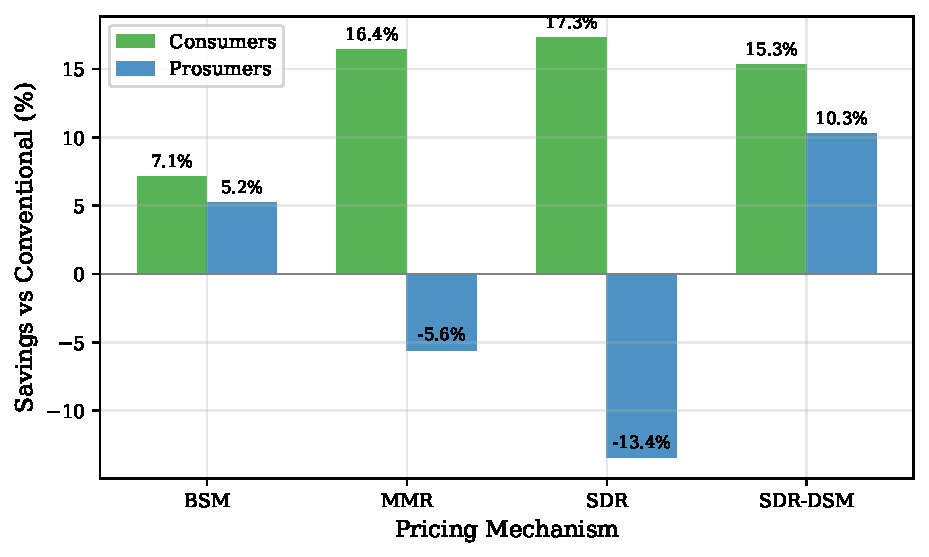
\includegraphics[width=\columnwidth]{fig_savings_by_group.pdf}
    \caption{Consumer and prosumer cost deltas by mechanism, illustrating the equity advantage of SDR-DSM.}
    \label{fig:savings_group}
\end{figure}

\subsection{Parametric Sensitivity Analysis}

\subsubsection{Community Size Sweep}

Table~\ref{tab:community_sweep} presents results across community sizes from $N=7$ to $N=50$. SDR-DSM consistently achieves the highest savings and fairness across all sizes. Notably, fairness improves with community size (from $\mathcal{F}=0.84$ at $N=7$ to $\mathcal{F}=0.97$ at $N=50$), as larger communities provide greater load diversity for the SDR pricing mechanism to exploit.

\begin{table}[t]
\caption{Community Size Sweep: SDR-DSM Performance}
\label{tab:community_sweep}
\centering
\footnotesize
\begin{tabular}{lcccc}
\toprule
\textbf{Config} & \textbf{CS (\%)} & $\Delta_{\mathcal{C}}$ \textbf{(\%)} & $\Delta_{\mathcal{P}}$ \textbf{(\%)} & $\mathcal{F}$ \\
\midrule
2C+5P ($N=7$) & 18.55 & 20.35 & 14.72 & 0.84 \\
3C+7P ($N=10$) & 15.35 & 18.15 & 11.98 & 0.80 \\
5C+15P ($N=20$) & 14.93 & 16.93 & 13.34 & 0.88 \\
10C+20P ($N=30$) & 13.64 & 15.38 & 11.18 & 0.84 \\
15C+35P ($N=50$) & 14.50 & 14.16 & 14.90 & \textbf{0.97} \\
\bottomrule
\end{tabular}
\end{table}

Fig.~\ref{fig:community_sweep} visualizes all mechanisms across community sizes, demonstrating SDR-DSM's consistent dominance.

\begin{figure}[t]
    \centering
    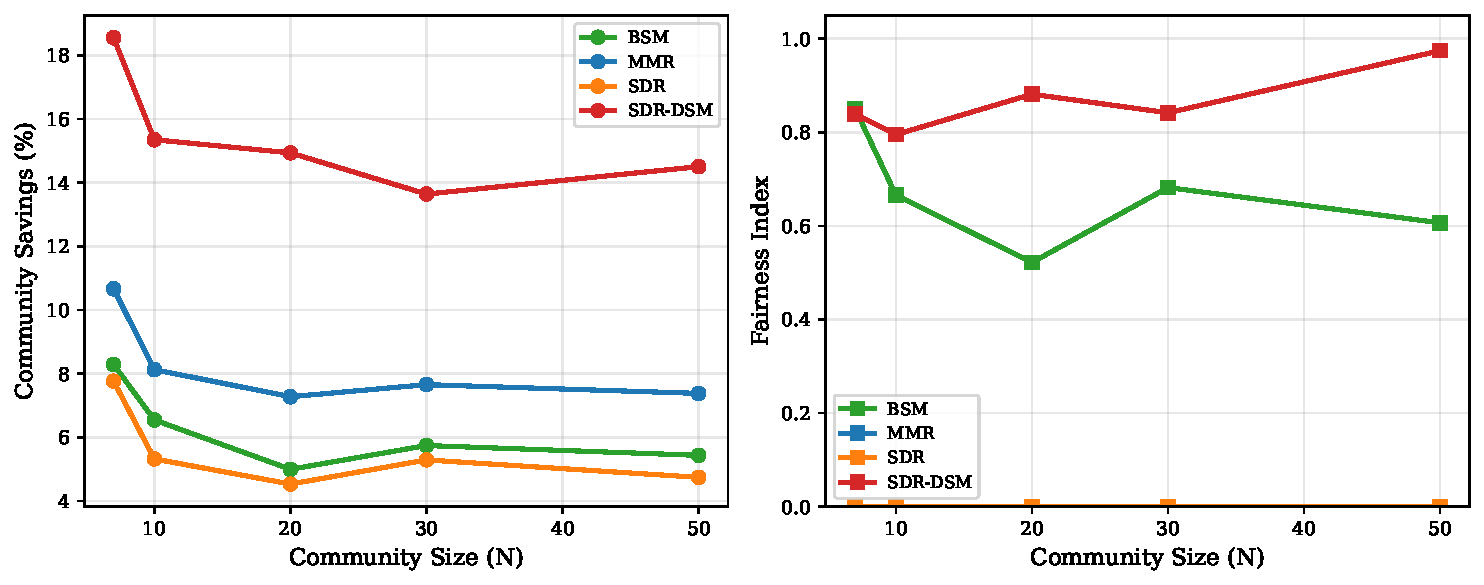
\includegraphics[width=\columnwidth]{fig_community_sweep.pdf}
    \caption{Community savings and fairness across community sizes ($N=7$--50) for all mechanisms.}
    \label{fig:community_sweep}
\end{figure}

\subsubsection{DSM Aggressiveness ($\alpha$) Sensitivity}

Fig.~\ref{fig:alpha} shows the impact of the discomfort coefficient $\alpha$ on SDR-DSM performance. For $\alpha \leq 1.0$, community savings plateau at approximately 13.5\% because load shifting is constrained by the $\pm$50\% bounds rather than the penalty---the optimization hits the physical limits regardless of further penalty reduction. For $\alpha > 2.0$, savings progressively degrade: at $\alpha = 20.0$, savings drop to 7.7\% (approaching static SDR performance) as the penalty dominates and load shifting becomes negligible. The energy shifted decreases from 447~kWh (bound-limited regime) to 150~kWh at $\alpha = 20.0$.

\begin{figure}[t]
    \centering
    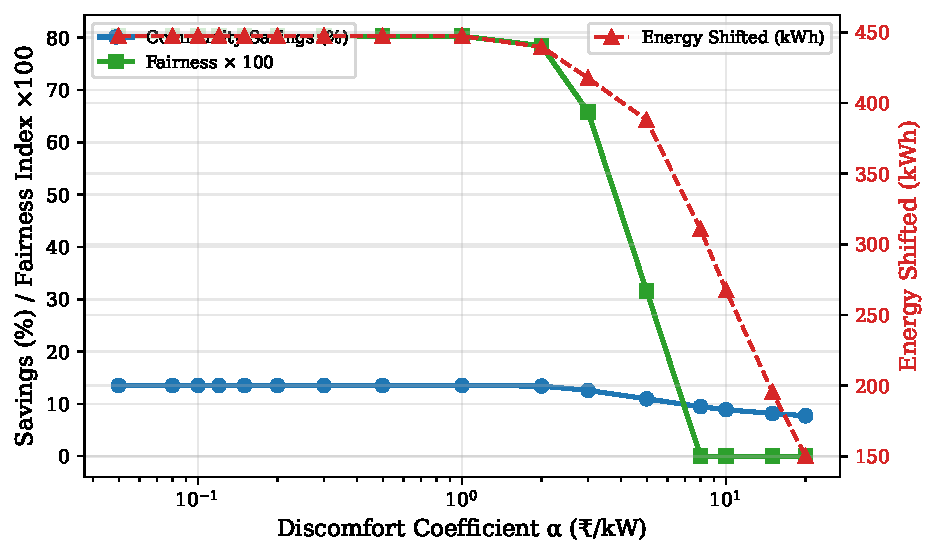
\includegraphics[width=\columnwidth]{fig_alpha_sensitivity.pdf}
    \caption{Impact of DSM discomfort coefficient $\alpha$ on community savings and energy shifted ($N=20$).}
    \label{fig:alpha}
\end{figure}

\begin{remark}
The plateau for $\alpha \leq 1.0$ indicates that the $\pm$50\% load bounds are the binding constraint in this regime, not the quadratic penalty. This suggests that even modest demand response capability (any $\alpha < 1.0$) achieves near-maximum benefit, reducing the sensitivity to accurate estimation of household discomfort parameters.
\end{remark}

\subsubsection{Prosumer Ratio Sweep}

Fig.~\ref{fig:prosumer_ratio} shows how community composition affects mechanism performance (fixed $N=30$, prosumer fraction 30\%--90\%). Key findings:
\begin{itemize}
    \item SDR-DSM savings increase monotonically with prosumer fraction: from 8.1\% (30\% prosumers) to 16.8\% (90\% prosumers), as more local generation creates greater P2P trading opportunity.
    \item Fairness under SDR-DSM remains high ($\mathcal{F} > 0.69$) across all compositions, with optimal equity at 80\% prosumers ($\mathcal{F} = 0.91$).
    \item MMR transitions from prosumer-penalizing ($\Delta_\mathcal{P} = -5.3$\% at 30\%) to mildly beneficial ($\Delta_\mathcal{P} = +1.8$\% at 90\%) but with reduced consumer benefit at high prosumer fractions.
    \item BSM maintains moderate fairness but consistently lower savings than SDR-DSM.
\end{itemize}

\begin{figure}[t]
    \centering
    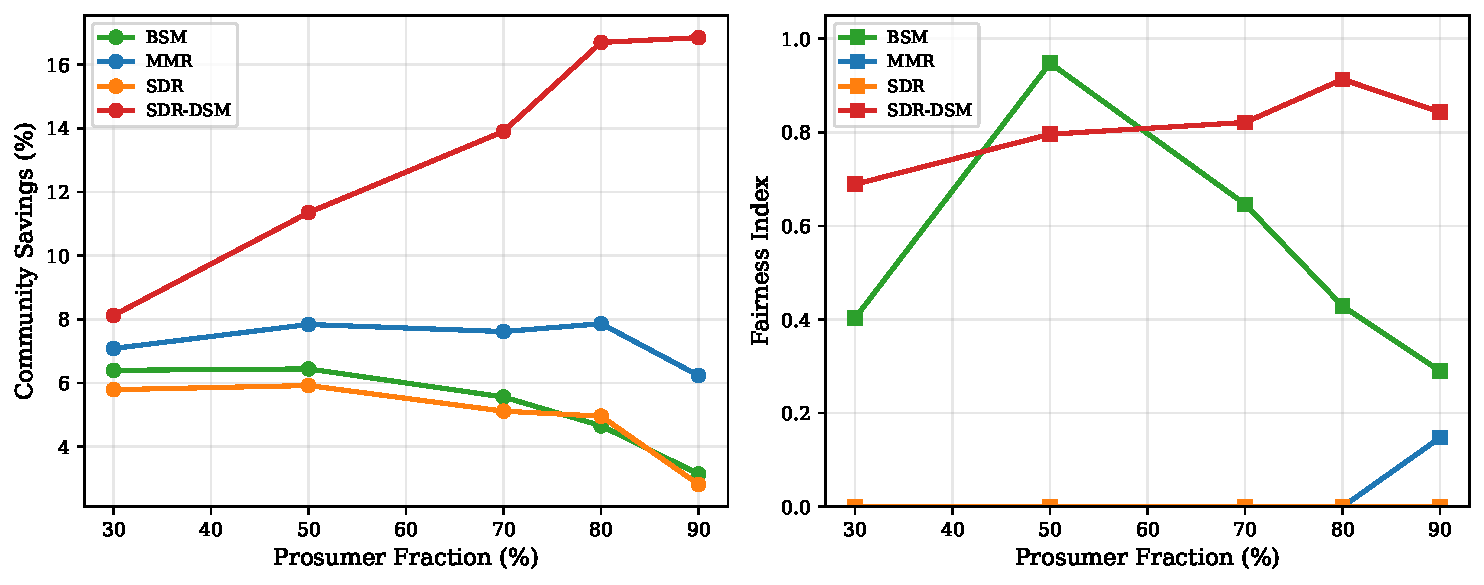
\includegraphics[width=\columnwidth]{fig_prosumer_ratio.pdf}
    \caption{Mechanism performance vs. prosumer fraction ($N=30$): community savings and fairness.}
    \label{fig:prosumer_ratio}
\end{figure}

\subsubsection{Tariff Spread Sensitivity}

Fig.~\ref{fig:tariff} examines how the grid buy--sell spread affects P2P market viability ($N=20$, spread from \rupee~1.0 to \rupee~7.5/kWh). The spread between $\bar{\pi}^{\text{buy}}$ and $\bar{\pi}^{\text{sell}}$ defines the P2P price corridor width. With a narrow spread (\rupee~1.0), all mechanisms achieve modest savings (3--7\%) because the price corridor provides limited room for P2P trading to create value. As the spread widens, SDR-DSM savings increase to 17.7\% at \rupee~7.5 spread. Interestingly, SDR-DSM fairness shows non-monotonic behavior: it peaks at narrow spreads (where load shifting is less aggressive) and decreases at very wide spreads where prosumers benefit disproportionately from higher export value.

\begin{figure}[t]
    \centering
    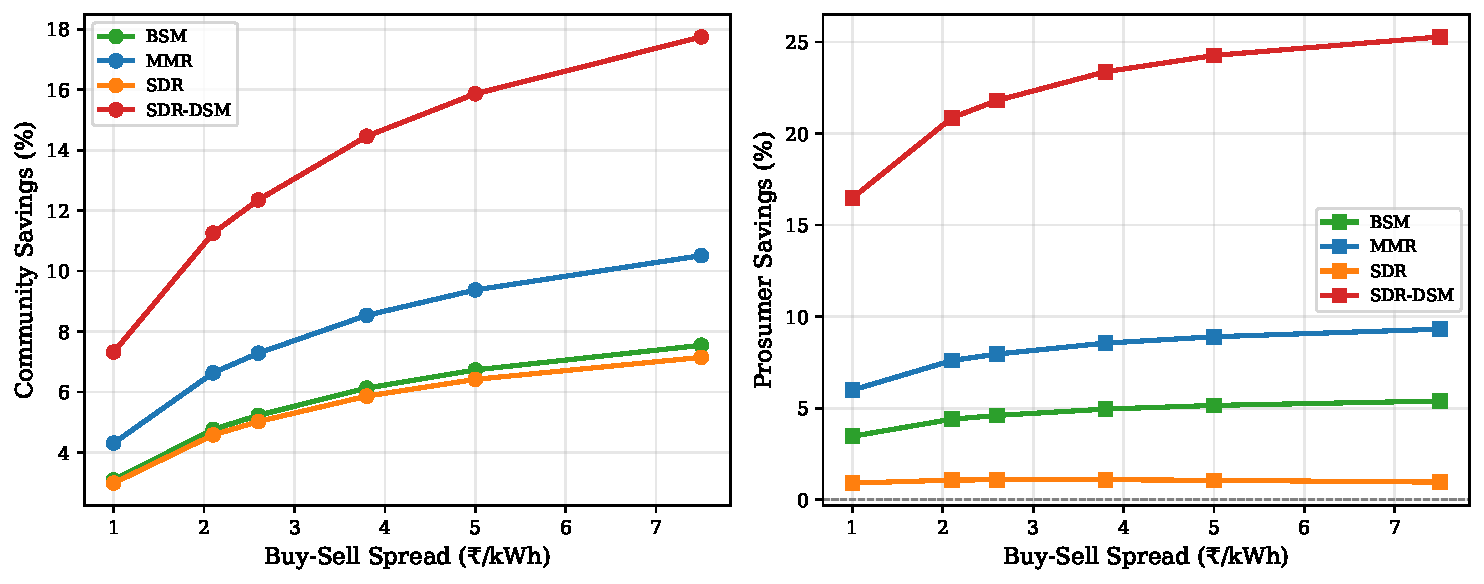
\includegraphics[width=\columnwidth]{fig_tariff_spread.pdf}
    \caption{Impact of grid tariff buy--sell spread on mechanism performance ($N=20$).}
    \label{fig:tariff}
\end{figure}

Table~\ref{tab:tariff} summarizes the tariff sensitivity results for SDR-DSM, showing that wider spreads favor prosumers while narrower spreads produce more equitable outcomes. Note that the tariff sweep uses uniform tariffs across all households, whereas the primary case (Table~\ref{tab:economics}) uses heterogeneous per-household tariffs drawn from a distribution, which accounts for the slight difference at similar nominal spread values.

\begin{table}[t]
\caption{Tariff Spread Sensitivity: SDR-DSM ($N=20$, 8C+12P)}
\label{tab:tariff}
\centering
\footnotesize
\begin{tabular}{lcccc}
\toprule
\textbf{Spread (\rupee/kWh)} & \textbf{CS (\%)} & $\Delta_{\mathcal{C}}$ (\%) & $\Delta_{\mathcal{P}}$ (\%) & $\mathcal{F}$ \\
\midrule
1.0 (Narrow) & 7.32 & 2.86 & 16.48 & 0.30 \\
2.1 & 11.26 & 4.93 & 20.85 & 0.38 \\
2.6 (Default) & 12.36 & 5.60 & 21.80 & 0.41 \\
3.8 & 14.46 & 7.04 & 23.37 & 0.46 \\
5.0 & 15.87 & 8.12 & 24.26 & 0.50 \\
7.5 (Wide) & 17.75 & 9.79 & 25.27 & 0.56 \\
\bottomrule
\end{tabular}
\end{table}

\subsection{Real Data Validation}

\subsubsection{Dataset Characteristics}

Fig.~\ref{fig:real_profiles} shows the average daily load profile from the 56 real Indian meters. The real data exhibits a distinct evening-dominated consumption pattern typical of Indian residential households: low nighttime base load (0.1--0.2~kW), gradual morning ramp, and a pronounced evening peak (18:00--22:00) driven by lighting, cooking, and entertainment loads. Compared to synthetic profiles, real data shows: (i)~higher heterogeneity between households (coefficient of variation $\approx$0.8 vs. 0.3 for synthetic), (ii)~sharper evening peaks, and (iii)~lower daytime base loads.

\begin{figure}[t]
    \centering
    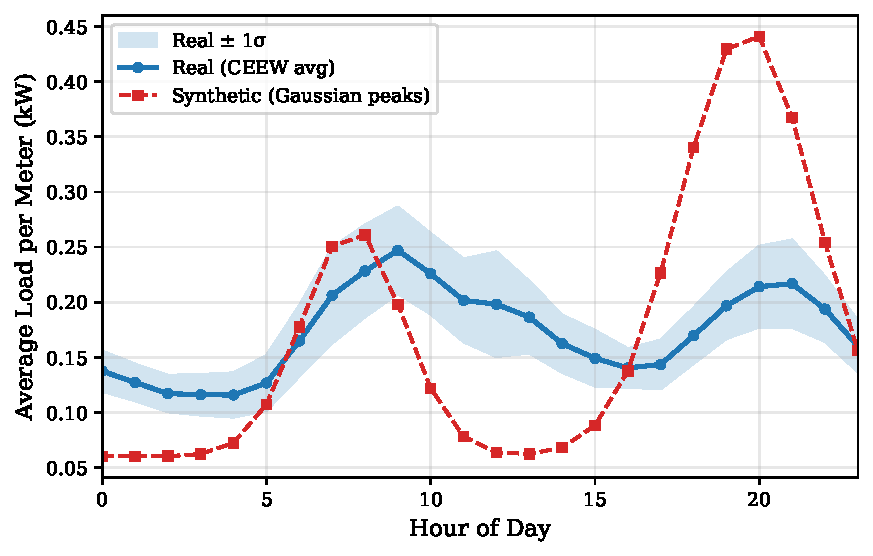
\includegraphics[width=\columnwidth]{fig_real_load_profiles.pdf}
    \caption{Average daily load profile from 56 real Indian smart meters (CEEW dataset) with variability band ($\pm$1 std. dev.).}
    \label{fig:real_profiles}
\end{figure}

\subsubsection{Load Reshaping on Real Data}

Fig.~\ref{fig:real_aggregate} shows the community aggregate power profile for all 56 real meters under SDR-DSM pricing. The adjusted load shifts substantially toward midday PV generation: peak adjusted demand occurs around 12:00 (coinciding with maximum PV output) rather than the evening peak of the reference profile. This reduces the surplus exported to the grid and increases local self-consumption. Compared to synthetic profiles (Fig.~\ref{fig:aggregate}), the real-data community exhibits a flatter reference profile without the pronounced twin-peak structure, reflecting the diversity of Indian household consumption patterns.

\begin{figure}[t]
    \centering
    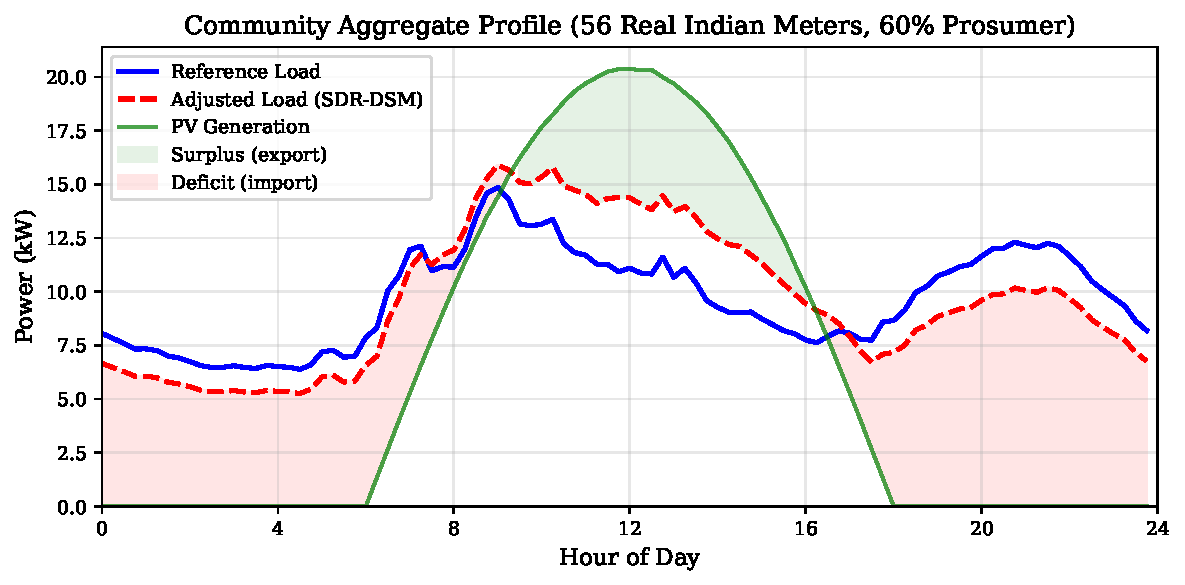
\includegraphics[width=\columnwidth]{fig_real_aggregate_reshaping.pdf}
    \caption{Community aggregate profile for 56 real Indian meters (60\% prosumer): DSM shifts demand toward midday PV generation, reducing grid exports.}
    \label{fig:real_aggregate}
\end{figure}

Fig.~\ref{fig:real_reshaping} presents individual load reshaping for representative households. Prosumer~A (high PV capacity) increases midday consumption by 30--50\% while reducing early morning and late evening loads. Prosumer~B (medium PV) shows a similar but more moderate pattern. Consumer~C, despite lacking PV, exhibits mild load shifting toward midday hours when P2P prices are lowest---demonstrating that SDR-DSM price signals benefit all participants, not just prosumers.

\begin{figure}[t]
    \centering
    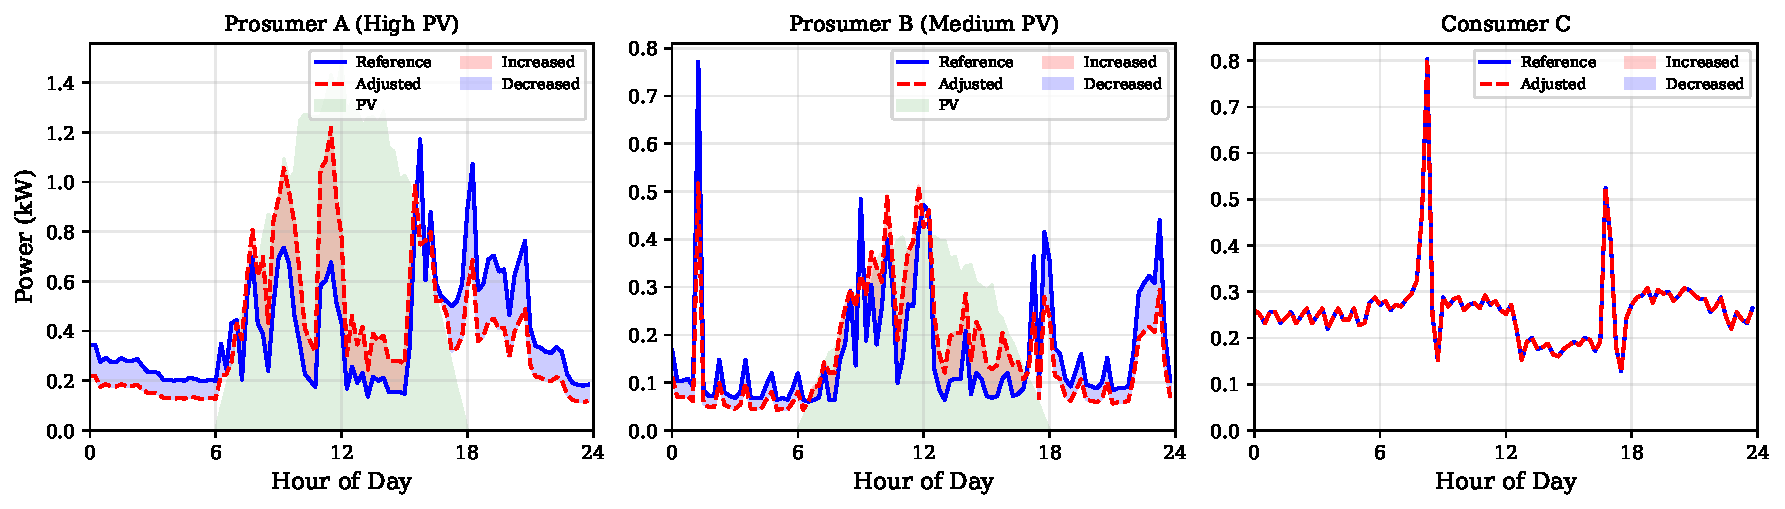
\includegraphics[width=\columnwidth]{fig_real_individual_reshaping.pdf}
    \caption{Individual load reshaping under SDR-DSM for real Indian households: prosumers shift load to coincide with PV generation (green shading), consumer responds to low midday P2P prices.}
    \label{fig:real_reshaping}
\end{figure}

\subsubsection{Mechanism Performance on Real Data}

Table~\ref{tab:real_results} presents mechanism performance on real data across different prosumer fractions (56 meters, 30 days). SDR-DSM consistently achieves the highest savings across all compositions, with savings increasing from 11.4\% (20\% prosumers) to 30.1\% (80\% prosumers). Fairness is particularly high for balanced compositions: $\mathcal{F} = 0.999$ at 40\% prosumers, indicating near-perfect equity between consumer and prosumer groups.

\begin{table}[t]
\caption{Real Data: Mechanism Performance by Prosumer Fraction (56 Meters)}
\label{tab:real_results}
\centering
\footnotesize
\begin{tabular}{llcccc}
\toprule
\textbf{Config} & \textbf{Mech.} & \textbf{CS (\%)} & $\Delta_{\mathcal{C}}$ (\%) & $\Delta_{\mathcal{P}}$ (\%) & $\mathcal{F}$ \\
\midrule
\multirow{4}{*}{20\% P} & BSM & 14.25 & 7.95 & 54.59 & 0.25 \\
 & MMR & 12.95 & 10.70 & 27.33 & 0.56 \\
 & SDR & 10.15 & 13.73 & $-$12.77 & $\approx$0 \\
 & SDR-DSM & \textbf{11.39} & 10.29 & 18.45 & \textbf{0.72} \\
\midrule
\multirow{4}{*}{40\% P} & BSM & 17.00 & 11.58 & 29.94 & 0.56 \\
 & MMR & 16.06 & 15.98 & 16.24 & 0.99 \\
 & SDR & 12.64 & 20.78 & $-$6.85 & $\approx$0 \\
 & SDR-DSM & \textbf{19.22} & 19.23 & 19.20 & \textbf{$\approx$1.00} \\
\midrule
\multirow{4}{*}{60\% P} & BSM & 18.06 & 13.24 & 22.15 & 0.75 \\
 & MMR & 18.06 & 18.91 & 17.33 & 0.96 \\
 & SDR & 12.76 & 23.52 & 3.63 & 0.27 \\
 & SDR-DSM & \textbf{24.48} & 22.86 & 25.85 & \textbf{0.94} \\
\midrule
\multirow{4}{*}{80\% P} & BSM & 17.23 & 15.31 & 17.71 & 0.93 \\
 & MMR & 19.95 & 22.54 & 19.31 & 0.92 \\
 & SDR & 12.13 & 26.99 & 8.42 & 0.48 \\
 & SDR-DSM & \textbf{30.15} & 26.69 & 31.01 & \textbf{0.93} \\
\bottomrule
\end{tabular}
\end{table}

Fig.~\ref{fig:real_sweep} visualizes the real-data prosumer fraction sweep, showing that SDR-DSM's advantage increases with prosumer fraction as more local generation enables greater P2P value creation.

\begin{figure}[t]
    \centering
    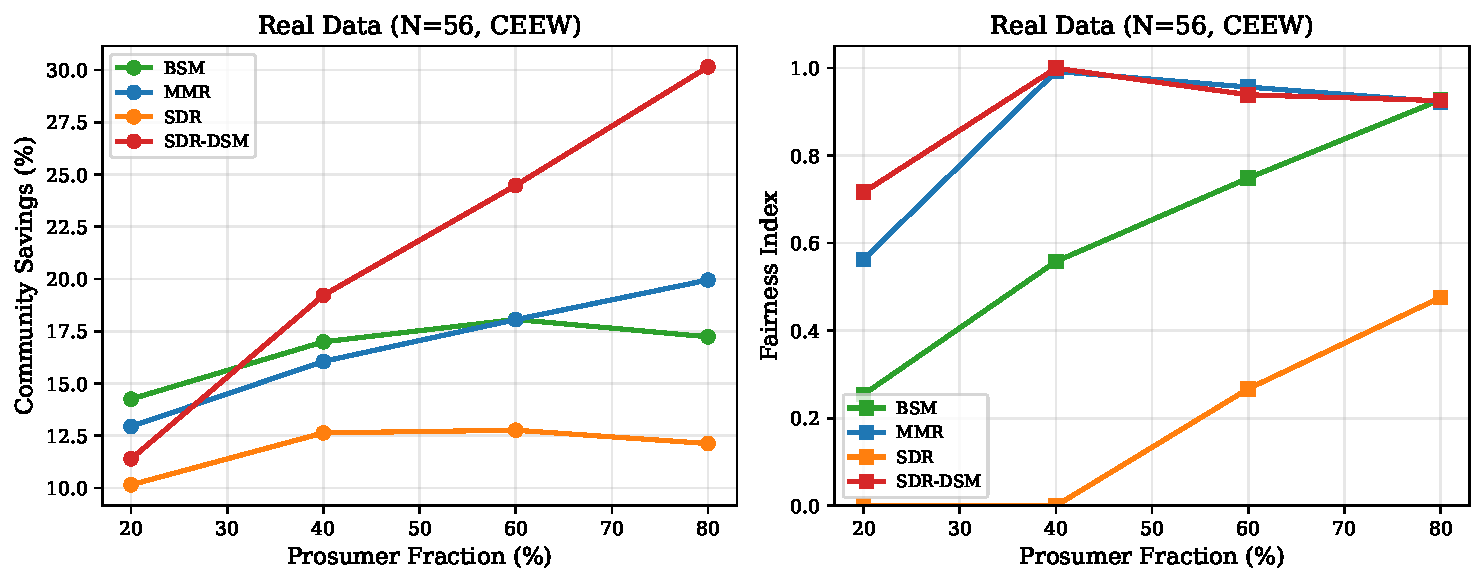
\includegraphics[width=\columnwidth]{fig_real_community_sweep.pdf}
    \caption{Real data validation: mechanism performance across prosumer fractions (56 meters, CEEW dataset).}
    \label{fig:real_sweep}
\end{figure}

\subsubsection{Synthetic vs. Real Data Comparison}

Table~\ref{tab:comparison} compares key metrics between synthetic and real data at approximately matched community compositions. The real-data results generally show higher savings than synthetic, attributable to: (i)~greater load heterogeneity providing more trading opportunities, (ii)~sharper peak/off-peak transitions creating larger SDR variations, and (iii)~lower daytime base loads making solar surplus relatively larger. The fairness improvement in real data ($\mathcal{F} = 0.94$--$1.00$ vs. $0.80$--$0.88$ synthetic) suggests that real household diversity actually benefits the SDR-DSM mechanism.

\begin{table}[t]
\caption{Synthetic vs. Real Data: SDR-DSM Comparison}
\label{tab:comparison}
\centering
\footnotesize
\begin{tabular}{lcccc}
\toprule
\textbf{Dataset} & \textbf{CS (\%)} & $\Delta_{\mathcal{C}}$ (\%) & $\Delta_{\mathcal{P}}$ (\%) & $\mathcal{F}$ \\
\midrule
Synthetic ($N=20$, 5C+15P) & 14.93 & 16.93 & 13.34 & 0.88 \\
Real (56 meters, 40\%P) & 19.22 & 19.23 & 19.20 & $\approx$1.00 \\
\midrule
Synthetic ($N=30$, 10C+20P) & 13.64 & 15.38 & 11.18 & 0.84 \\
Real (56 meters, 60\%P) & 24.48 & 22.86 & 25.85 & 0.94 \\
\bottomrule
\end{tabular}
\end{table}

%====================================================================
\section{Discussion}\label{sec:discussion}

\subsection{Policy Implications for Indian DISCOMs}

The results have direct implications for Indian energy policy:
\begin{itemize}
    \item \textbf{Tariff design}: The tariff spread sensitivity analysis shows that current Indian DISCOM spreads (\rupee~2.5--3.0/kWh typical) create sufficient P2P value to incentivize community formation without excessive complexity.
    \item \textbf{Community composition}: The prosumer ratio analysis suggests that communities with 40--60\% prosumers achieve optimal balance between savings magnitude and equity. Policy incentives could target this composition range.
    \item \textbf{DSM integration}: The $\alpha$ sensitivity results indicate that even modest demand flexibility (any $\alpha < 1.0$) captures near-maximum benefit, suggesting that basic time-of-use awareness---achievable through simple app-based notifications---suffices without requiring full home automation.
\end{itemize}

\subsection{Scalability Considerations}

The framework's computational complexity is $\mathcal{O}(N \cdot H \cdot k_{\max})$ per settlement, dominated by individual quadratic programs (closed-form solutions given prices). The community size sweep ($N=7$ to $N=50$) confirms that convergence behavior and fairness properties are robust to scaling. Communication requirements are modest: each iteration requires only aggregate power quantities from the ESP to participants (broadcast) and individual load schedules from participants to ESP (unicast).

\subsection{Limitations}

The present study has several limitations:
\begin{itemize}
    \item Battery energy storage systems (BESS) are not modeled; their inclusion would enable temporal arbitrage and potentially improve savings further.
    \item PV generation for real-data validation uses synthetic profiles rather than co-located irradiance measurements.
    \item The quadratic inconvenience cost model, while widely adopted, may not perfectly represent all household preference structures.
    \item A single flat tariff structure is used; time-of-use tariffs common in some Indian DISCOM jurisdictions would modify the P2P price corridor.
\end{itemize}

The copper-plate (lossless bus) network assumption is a deliberate architectural choice, consistent with the settlement-layer literature~\cite{liu2017, long2017, alfaverh2023}. The framework operates at the economic settlement layer: pricing mechanisms determine cost allocation given aggregate power quantities, independent of the physical network topology. Introducing distribution network constraints (voltage limits, line thermal ratings) would make results deployment-specific---dependent on feeder lengths, transformer ratings, and household spatial placement---destroying the topological symmetry that enables general community composition analysis. Moreover, since all mechanisms compared share the same physical flows, network losses would affect absolute costs proportionally across mechanisms without altering the relative rankings that are the focus of this study.

%====================================================================
\section{Conclusion}\label{sec:conclusion}

This paper presented a modular comparative framework for P2P energy trading in community microgrids, evaluating five settlement mechanisms under standardized conditions with both synthetic profiles and real Indian smart meter data. The key findings are:

\begin{enumerate}
    \item SDR-DSM consistently achieves the highest community savings among all mechanisms tested, ranging from 7.3\% (narrow tariff spread) to 30.1\% (real data, high prosumer fraction), while MMR and static SDR systematically penalize prosumers ($\mathcal{F} \to 0$). For the primary synthetic case ($N=20$), SDR-DSM achieves 13.5\% savings with $\mathcal{F} = 0.80$.
    \item Equilibrium existence is guaranteed by the Brouwer Fixed Point Theorem, and the distributed iterative algorithm with damped updates ($\gamma = 0.3$) converges within 8 iterations across all configurations tested ($N = 7$--$50$, $\alpha = 0.05$--$20.0$).
    \item Parametric sweeps reveal that: (a)~the $\pm$50\% load bounds are the binding DSM constraint for $\alpha \leq 1.0$; (b)~community fairness improves with size ($N=50$ achieves $\mathcal{F} = 0.97$); (c)~wider tariff spreads increase absolute savings but reduce equity ($\mathcal{F}$ decreases from 0.30 to 0.56 as spread widens from \rupee~1.0 to \rupee~7.5).
    \item Real-data validation using 56 Indian smart meters confirms and strengthens synthetic findings, with SDR-DSM achieving $\mathcal{F} \approx 1.00$ at 40\% prosumer composition and 30.1\% savings at 80\% prosumers---real household heterogeneity benefits rather than hinders the mechanism.
\end{enumerate}

Future work will extend the framework with BESS and vehicle-to-grid (V2G) modules for temporal energy arbitrage, stochastic optimization for PV and load forecast uncertainty, and field pilot studies with real prosumer communities in Indian urban settings. For deployment-specific studies, incorporating ACOPF network constraints would enable distribution-network-aware P2P trading where voltage and thermal limits are binding; however, such extensions necessarily sacrifice the topology-independent generalizability demonstrated here.

%====================================================================
\appendix
\section{Energy Allocation in SDR Pricing}\label{app:allocation}

At each time slot $t$, the P2P traded energy is:
\begin{equation}
    E_t^{\text{P2P}} = \min(P_t^{\text{buy}}, P_t^{\text{sell}}) \cdot \Delta t
\end{equation}

For importing participants ($P_{n,t}^{\text{net}} > 0$):
\begin{equation}
    E_{n,t}^{\text{P2P,buy}} = \frac{P_{n,t}^{\text{im}}}{P_t^{\text{buy}}} \cdot E_t^{\text{P2P}}, \quad E_{n,t}^{\text{grid,buy}} = P_{n,t}^{\text{im}} \cdot \Delta t - E_{n,t}^{\text{P2P,buy}}
\end{equation}

The individual bill for importer $n$ at slot $t$:
\begin{equation}
    B_{n,t} = E_{n,t}^{\text{P2P,buy}} \cdot \pi_t^{\text{int,buy}} + E_{n,t}^{\text{grid,buy}} \cdot \bar{\pi}^{\text{buy}}
\end{equation}

For exporting participants ($P_{n,t}^{\text{net}} < 0$):
\begin{equation}
    E_{n,t}^{\text{P2P,sell}} = \frac{P_{n,t}^{\text{ex}}}{P_t^{\text{sell}}} \cdot E_t^{\text{P2P}}, \quad E_{n,t}^{\text{grid,sell}} = P_{n,t}^{\text{ex}} \cdot \Delta t - E_{n,t}^{\text{P2P,sell}}
\end{equation}

Revenue for exporter $n$:
\begin{equation}
    R_{n,t} = E_{n,t}^{\text{P2P,sell}} \cdot \pi_t^{\text{int,sell}} + E_{n,t}^{\text{grid,sell}} \cdot \bar{\pi}^{\text{sell}}
\end{equation}

%====================================================================
\bibliography{sn-bibliography}

\end{document}
